\xiti
\begin{xiaotis}
\begin{enhancedline}

\xiaoti{定圆 $O$ 的半径是 4 厘米, 动圆 $P$ 的半径是 1 厘米。}
\begin{xiaoxiaotis}

    \xxt{设 $\yuan\,P$ 和 $\yuan\,O$ 相外切。 那么点 $P$ 与点 $O$ 的距离是多少? 点 $P$ 可以在什么样的线上移动?}

    \xxt{设 $\yuan\,P$ 和 $\yuan\,O$相内切呢?}

\end{xiaoxiaotis}

\xiaoti{分别以 2 厘米、2.5 厘米、4 厘米为半径作圆,使它们两两外切。}

\xiaoti{经过相交两圆的一个交点,作两圆的公共弦的垂线。求证:这条直线上被两圆所截得的线段等于圆心距的二倍。}

\xiaoti{已知: $\yuan\,O_1$ 和 $\yuan\,O_2$ 相交于点 $A$ 和 $B$,
    经过点 $A$ 的直线分别交两圆于点 $C$ 和 $D$,
    经过点 $B$ 的直线分别交两圆于点 $E$ 和 $F$, 且 $CD \pingxing EF$。求证:
}
\begin{xiaoxiaotis}

    \xxt{$CD = EF$;}

    \xxt{$CE = DF$。}

\end{xiaoxiaotis}

\xiaoti{已知: $\yuan\,O$ 和 $\yuan\,O'$ 外切于点 $A$, 经过点 $A$ 作直线 $BC$ 和 $DE$,
    $BC$ 交 $\yuan\,O$ 于点 $B$、交 $\yuan\,O'$ 于点 $C$,
    $DE$ 交 $\yuan\,O$ 于点 $D$、交 $\yuan\,O'$ 于点 $E$。
    求证: $BD \pingxing CE$。
}

\xiaoti{经过相内切的两圆的切点 $A$ 作大圆的弦 $AD$、$AE$, 设 $AD$、$AE$ 分别和小圆相交于点 $B$、$C$。
    求证:$DE \pingxing BC$; $AB:AC = AD:AE$。
}

\xiaoti{已知两个圆相外切,它们的两条外公切线互相垂直,其中大圆的半径等于 5 cm。求小圆半径及外公切线长。}

\xiaoti{$\yuan\,O_1$ 和 $\yuan\,O_2$ 相交于点 $B$ 和 $C$,
    $A$ 是 $\yuan\,O_1$ 上另一点, $AT$ 是 $\yuan\,O_1$ 的切线,
    又直线 $AB$ 与 $AC$ 分别交 $\yuan\,O_2$ 于点 $D$ 和 $E$。
    求证:$AT \pingxing DE$。
}

\xiaoti{用半径 $R = 8$ mm、 $r = 5$ mm 的钢球测量口小内大的内孔的直径 $D$。
    测得钢球顶点与孔口平面的距离分别为 $a = 12.5$ mm、$b = 8.3$ mm(如图),
    计算出内孔直径 $D$ 的大小(精确到 0.1 mm)。
}

\begin{figure}[htbp]
    \centering
    \begin{minipage}[b]{4.1cm}
        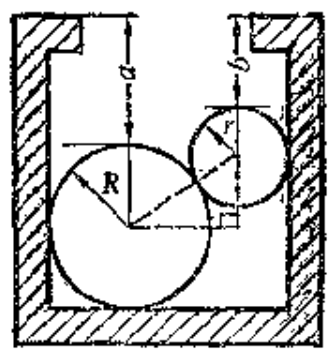
\includegraphics[width=4cm]{../pic/czjh2-ch7-xiti26-09.png}
        \caption*{}
        \caption*{(第 9 题)}
    \end{minipage}
    \qquad
    \begin{minipage}[b]{11cm}
        \begin{minipage}[b]{5.1cm}
            \centering
            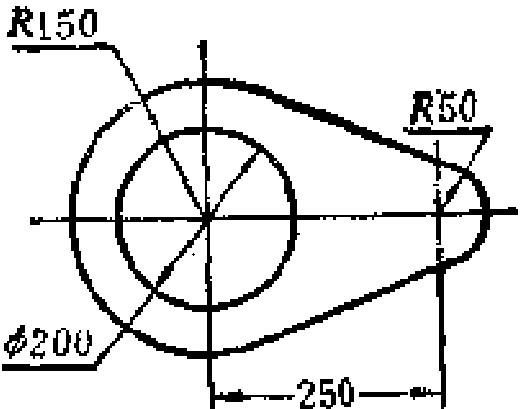
\includegraphics[width=5cm]{../pic/czjh2-ch7-xiti26-12-a.png}
            \caption*{甲}
        \end{minipage}
        \begin{minipage}[b]{5.8cm}
            \centering
            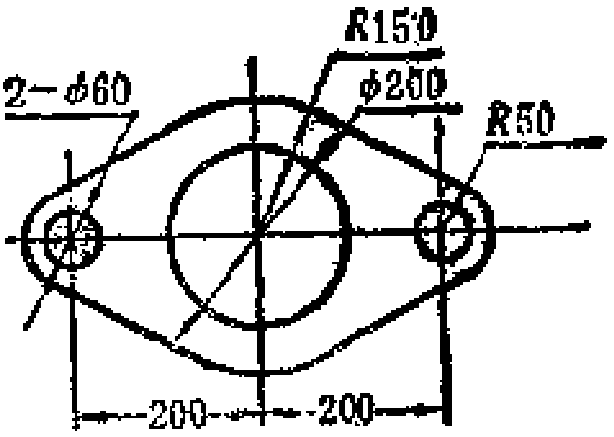
\includegraphics[width=5.7cm]{../pic/czjh2-ch7-xiti26-12-b.png}
            \caption*{乙}
        \end{minipage}
        \caption*{(第 12 题)}
    \end{minipage}
\end{figure}

\xiaoti{两圆半径为 38 mm和 22 mm, 圆心距为 65 mm。求}
\begin{xiaoxiaotis}

    \xxt{内公切线长;}

    \xxt{内公切线与连心线的夹角。}

\end{xiaoxiaotis}

\xiaoti{求证:}
\begin{xiaoxiaotis}

    \xxt{两圆的外公切线的四个切点在同一个圆上;}

    \xxt{两圆的内公切线的四个切点在同一个圆上。}
\end{xiaoxiaotis}

\xiaoti{按 $1:5$ 的比例尺,作出下列图样。}

% \begin{figure}[htbp]
%     \centering
%     \begin{minipage}[b]{7cm}
%         \centering
%         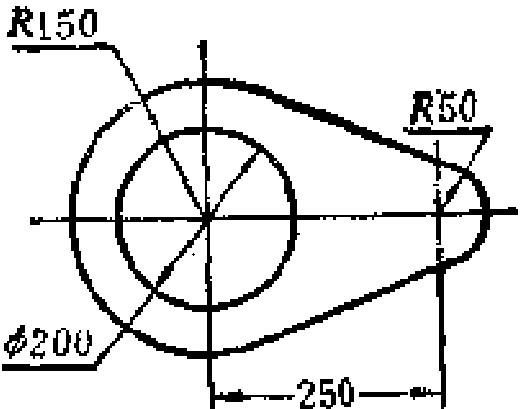
\includegraphics[width=5cm]{../pic/czjh2-ch7-xiti26-12-a.png}
%         \caption*{甲}
%     \end{minipage}
%     \begin{minipage}[b]{7cm}
%         \centering
%         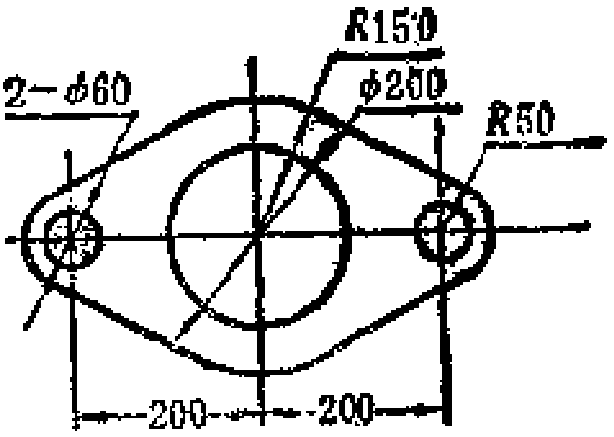
\includegraphics[width=5.7cm]{../pic/czjh2-ch7-xiti26-12-b.png}
%         \caption*{乙}
%     \end{minipage}
%     \caption*{(第 12 题)}
% \end{figure}

\xiaoti{如图, $ABCD$ 是正方形,曲线 $DEFG\cdots$ 叫做 “正方形的渐开线”。
    其中 $\yuanhu{DE}$、$\yuanhu{EF}$、$\yuanhu{FG}$、$\yuanhu{GH}$、$\cdots$
    的圆心依次按 $A$、$B$、$C$、$D$ 循环,它们依次相连接,取 $AB = 10$ mm,作图。
}

\begin{figure}[htbp]
    \centering
    \begin{minipage}[b]{7cm}
        \centering
        \begin{tikzpicture}[scale=.9] % 复杂
    \pgfmathsetmacro{\a}{0.6}

    % 绘制“正方形的渐开线”
    \tkzDefPoints{0/0/p0, -\a/0/p1, -\a/\a/p2, 0/\a/p3}
    \foreach \i in {4,5, ..., 8} {
        \pgfmathsetmacro{\o}{int(mod(\i, 4))}
        \pgfmathsetmacro{\s}{int(\i - 1)}
        \tkzDefPointBy[rotation=center {p\o} angle -90]({p\s})  \tkzGetPoint{{p\i}}
        \tkzDrawArc({p\o},{p\i})({p\s})
    }
    % 绘制最后的一小节
    \tkzDefPointBy[rotation=center p0 angle -50](p8)  \tkzGetPoint{X}
    \tkzDrawArc({p0},X)(p8)

    % 绘制正方形及其延长线
    \tkzDrawLine[add=0 and 0.2](p0, p7)
    \tkzDrawLine[add=0 and 0.2](p1, p8)
    \tkzDrawLine[add=0 and 0.2](p2, p5)
    \tkzDrawLine[add=0 and 0.2](p3, p6)

    % 显示坐标点
    \tkzLabelPoint[below](p0){$A$}
    \tkzLabelPoint[left](p1){$B$}
    \tkzLabelPoint[above](p2){$C$}
    \tkzLabelPoint[above right](p3){$D$}
    \tkzLabelPoint[below right](p4){$E$}
    \tkzLabelPoint[below right](p5){$F$}
    \tkzLabelPoint[below left](p6){$G$}
    \tkzLabelPoint[above right](p7){$H$}
    \tkzLabelPoint[below right](p8){$K$}
\end{tikzpicture}


        \caption*{(第 13 题)}
    \end{minipage}
    \qquad
    \begin{minipage}[b]{7cm}
        \centering
        \begin{tikzpicture}
    % 由各圆两两相切,得: (R - r)^2 + (R/2)^2 = (R/2 + r)^2
    % 解得: r = R/3

    % 大圆
    \pgfmathsetmacro{\R}{3}
    \tkzDefPoints{0/0/A, \R/0/O, 2*\R/0/B}
    \tkzDrawSegment[thick](A,B)
    \tkzDrawArc[very thick](O,B)(A)
    \tkzDrawPoint(O)

    % 左侧的小圆 A
    \tkzDefPoints{0.5*\R/0/O_1}
    \tkzDrawArc[very thick](O_1,O)(A)
    \tkzDrawPoint(O_1)

    % 右侧的小圆 B
    \tkzDefPoints{1.5*\R/0/O_2}
    \tkzDrawArc[very thick](O_2,B)(O)
    \tkzDrawPoint(O_2)

    % 上方的小圆 C
    \pgfmathsetmacro{\r}{\R/3}
    \tkzDefPoints{\R/\R-\r/O_3, \R/\R/C}
    \tkzDrawCircle[very thick](O_3,C)
    \tkzDrawPoint(O_3)
\end{tikzpicture}

        \caption*{(第 14 题)}
    \end{minipage}
\end{figure}

\xiaoti{已知图中各圆两两相切, 大圆半径为 $R$。求各小圆的半径,并画出图形。}

\end{enhancedline}
\end{xiaotis}

